Important observation I wanted to highlight today:

\begin{tcolorbox}
In math, we work with \textit{functions} a lot. Recall the basic property of a function: it will take a value (a number, an animal, anything) and output another value (a letter of the alphabet, the number of the animal's legs, anything). Later on we will learn a more rigorous definition than that described above.
\end{tcolorbox}

Then a boolean expression is really a function. Each variable takes in either true or false, at which point we can \textit{evaluate} the expression and we get some boolean value (either true or false). Consider the expression
\[(p \land q) \lor r.\]
Then we can feed in any combination of trues or falses. For example, if $p \equiv T$, $q \equiv F$, and $r \equiv T$, then the expression above will evaluate these values to 
\[(T \land F) \lor T \equiv F \lor T \equiv T,\] or true.

A \textbf{truth table} then is really just a way of recording the output values of this function.

 \begin{enumerate}
   \item Create truth tables for the following expressions.

\begin{itemize}
    \item $p \land (\sim p)$ (This formula is called \textit{unsatisfiable}. Why is this?)
    \item $p \land T$ (Here, $T$ represents true. Similarly, $F$ represents false).
    \item $p \land F$
    \item $p \lor T$ and $p \lor F$.
\end{itemize}


   \begin{tcolorbox}
Two logical expressions are called \textbf{logically equivalent} if they have the same truth value given a set of truth values for each variable.

Equivalently, two logical expressions are logically equivalent if they have the same truth table.
\end{tcolorbox}
    \item Let's consider the logical expressions in problem 1 again. Figure out simpler expressions which are equivalent to these.
    \item Consider the following chunk of code. Here, \verb|var1|, \verb|var2| are boolean variables (ie, they are true or false).
\begin{verbatim}
    if (var1 && (var1 || var2)) { printf("She loves me!"); }
    else { printf("She loves me not..."); }
\end{verbatim}
Simplify the code.


    \item We have made it a point in this section that given a logical expression (or even an arithmetic expression), parentheses matter!

Build the truth tables for $(\sim a) \land b$ and $\sim (a \land b)$. Compare it to the viral facebook math problem below:

\begin{figure}[ht]
    \centering
    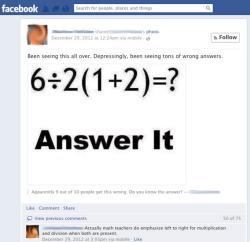
\includegraphics{Ch1/arithmetic.jpg}
    \caption{Viral Facebook Math Meme}
    \label{fig:arithmetic}
\end{figure}
    \item This problem mostly deals with the implies $(\implies)$ logical operator. The motivation behind this operator is that eventually we want to do \textbf{proofs}. That is, given a set of initial hypotheses, we want to make deductions and logically deduce that a conclusion is true. For example, eventually all of you will be able to prove, roughly stated:
\[(\text{$n$ is even}) \implies (\text{$n + 1$ is odd}).\]

Construct the truth tables for all the logical expressions below.
%I'll cover the first two bullets in class.
\begin{itemize}
    \item $p \implies (p \land q)$ and $p \implies (p \lor q)$.
    \item $(p \land q) \implies (p \lor q)$. This formula is an example of a \textit{tautology}.
    \item $(p \lor q) \implies (p \land q)$.
    \item $(p \implies q) \implies (p \iff q)$.
    \item $(p \iff q) \implies (p \implies q)$.
    \item $p \implies q \implies r$ and $p \implies r$.
\end{itemize}
 \end{enumerate}
